\chapter{METODOLOGI}
\label{chap:metodologi}

% Ubah bagian-bagian berikut dengan isi dari desain dan implementasi

Judul penelitian "Deteksi Helm Keselamatan Kerja Menggunakan CNN" mengikuti metode atau desain sistem berikut serta impelementasinya.


\section{Peralatan}
\label{sec:peralatan}

Dalam pengerjaan judul tugas akhir ini, terdapat beberapa peralatan dan bahan yang digunakan dalam rangka menyelesaikan penelitian ini mulai dari tools berupa software atau perangkat lunak hingga hardware atau perangkat keras. Berikut pemaparan dari alat - alat yang digunakan.

\begin{enumerate}[nolistsep]
  \item Computer Desktop 
  \item Google Colab
  \item Jetson Nano
  \item Webcam Nemesis NYK A-90 Everest
\end{enumerate}


\begin{longtable}{|c|c|c|}
  \caption{Spesifikasi Komputer Desktop}
  \label{tb:spesifikasikomputer}\\
  \hline
  % \rowcolor[HTML]{C0C0C0}
  \textbf{Tipe} & \textbf{Detail}  \\
  \hline
  \textit{Processor} & AMD Ryzen 5 2600 \\ 
  Memory             & 16 GB  \\
  Storage            & HDD 1TB SSD 1,256 TB\\
  Graphic Card       & NVIDIA GeForce GTX 1060 6GB \\
  Operating System   & Windows 10     \\
  CUDA               & CUDA version 11.2    \\              
  \hline
\end{longtable}

\begin{longtable}{|c|c|c|}
  \caption{Spesifikasi Jetson Nano}
  \label{tb:spesifikasijetsonano}\\
  \hline
  % \rowcolor[HTML]{C0C0C0}
  \textbf{Tipe} & \textbf{Detail}  \\
  \hline
  \textit{Processor} & Quad-core ARM Cortex-A57 MPCore processor \\ 
  Memory             & 4 GB 64-bit LPDDR4, 1600MHz 25.6 GB/s  \\
  Storage            & SDCARD 512 GB\\
  Graphic Card       & NVIDIA Maxwell architecture with 128 NVIDIA CUDA® cores \\
  Operating System   & Ubuntu     \\
  CUDA               & CUDA version 10.2.300    \\              
  \hline
\end{longtable}

\begin{longtable}{|c|c|c|}
  \caption{Spesifikasi Webcam Nemesis NYK A-90 Everest}
  \label{tb:spesifikasijetsonano}\\
  \hline
  % \rowcolor[HTML]{C0C0C0}
  \textbf{Tipe} & \textbf{Detail}  \\
  \hline
  Resolution         & 1920x1080 \\ 
  Max FPS            & 30 FPS  \\
  Other Detail       & Full 360 Degree Rotation \\
                      & Auto Focus \\
                      & Auto Exposure White Balance    \\
                     & Full HD Glass Lens    \\              
  \hline
\end{longtable}

\section{Desain Sistem}
\label{sec:desainsistem}

Judul untuk tugas akhir “Deteksi Helm Keselamatan Kerja Menggunakan CNN” ini berada dalam bidang computer vision atau visi komputer yang memiliki tujuan merancang sistem yang dapat mendeteksi penggunaan helm keselamatan kerja secara real-time. Menggunakan YOLOv5 yang merupakan versi terbaru dari YOLO (You Only Look Once) yang merupakan algoritma deteksi objek yang berbasis CNN (Convolutional Neural Network). Dataset yang digunakan berupa gambar - gambar personnel proyek yang mengenakan helm keselamatan kerja dan yang tidak. Gambar - gambar tersebut dikumpulkan dari beberapa sumber seperti dataset dari kaggle dan sumber lainnya.

\begin{figure}[ht]
  \centering
  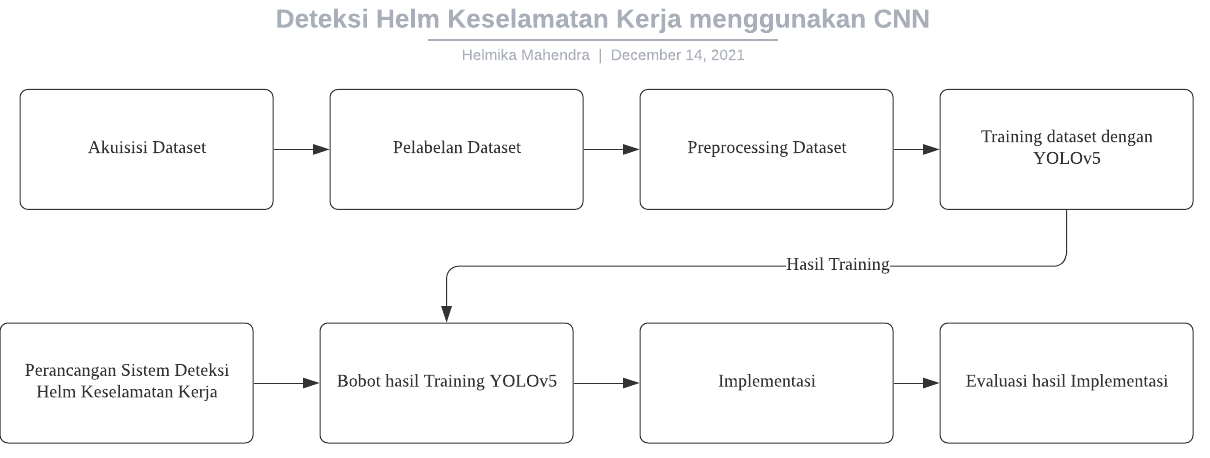
\includegraphics[width=1.0\textwidth]{gambar/Metodologi CNN.png}
  \caption{Bagan Umum Sistem}
  \label{fig:baganumumsistem}  
\end{figure}

\section{Alur Kerja}
\label{sec:alurkerja}

Prosedur pengerjaan dari judul tugas akhir ini dibagi menjadi beberapa tahap yang didasari dari metodologi yang sudah disusun seperti di gambar metodologi, yaitu :

\begin{enumerate}[nolistsep]
  \item Akuisi Dataset
  \item Pelabelan Dataset
  \item Preprocessing Dataset
  \item Training Dataset dengan Yolov5
  \item Perancangan Sistem Deteksi Helm Keselamatan Kerja
  \item Implementasi
  \item Evaluasi hasil implementasi
\end{enumerate}


\section{Akuisi Dataset}
\label{sec:akuisisidataset}

Dataset yang digunakan untuk training menggunakan Yolov5 berupa dataset berisi gambar - gambar yang mengandung personel lapangan proyek yang mengenakan helm dan yang tidak mengenakan helm. Untuk penelitian ini, dataset yang digunakan berasal dari dua sumber yaitu :

\begin{enumerate}
  \item Safety Helmet Detection oleh andrewmvd
  \par Dataset ini berisi 5000 gambar pekerja konstruksi yang meliputi orang yang menggunakan helm dan yang tidak menggunakan helm keselamatan kerja. Masin - masing
  gambar sudah diberi label ”helmet” dan ”head”. Format anotasi label nya berupa
  fromat PASCAL VOC yang disimpan dalam file .xml.   

  \begin{figure}[ht]
    \centering
    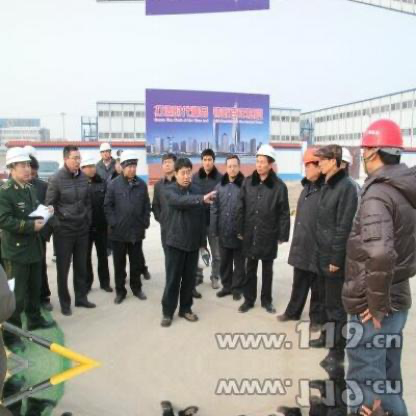
\includegraphics[width=0.3\textwidth]{gambar/sample_kaggle1/hard_hat_workers0.png}
    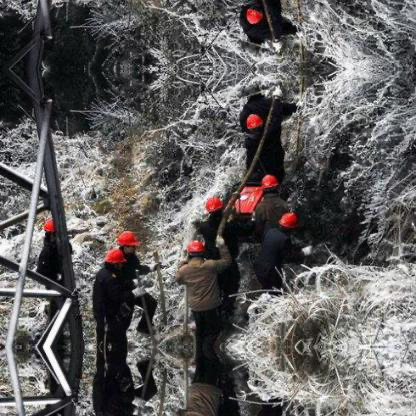
\includegraphics[width=0.3\textwidth]{gambar/sample_kaggle1/hard_hat_workers1.png}
    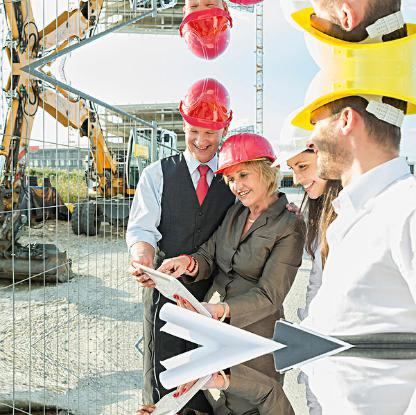
\includegraphics[width=0.3\textwidth]{gambar/sample_kaggle1/hard_hat_workers19.png}
    \caption{Dataset \emph{Safety Helmet Detection} oleh andrewmvd}
    \label{fig:datasethelmetdetectionpreview}  
  \end{figure}

  \item SampleERASTY2020 dataset oleh Muhammad Aditya Wicaksono
  \par Dataset ini berisi 8.867 gambar yang kandungannya serupa dengan dataset Safety Helmet 
  Detection oleh andrewmvd sebelumnya. Dataset ini juga sudah lengkap dengan annotasi nya tetapi 
  membutuhkan beberapa perubahan untuk disesuaikan dengan  metode trainingnya. 
  Selain itu, 8.867 gambar tersebut juga sudah termasuk hasil augmentasi seperti flip, 
  rotation, blur, dan noise.

  \begin{figure}[ht]
    \centering
    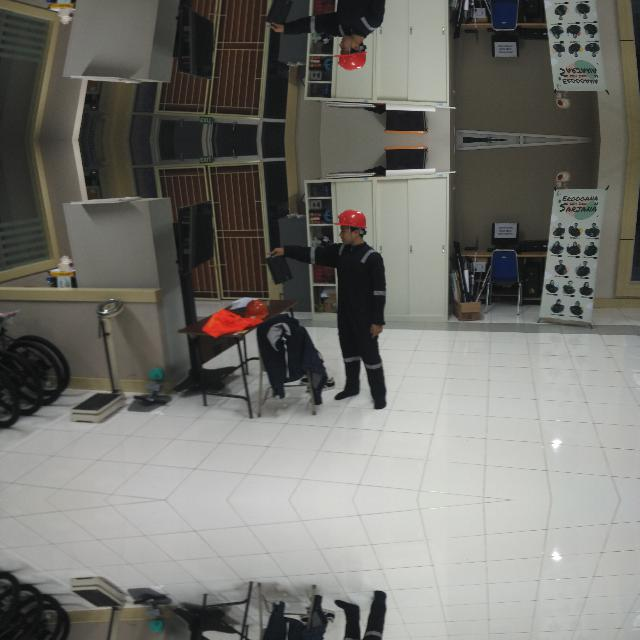
\includegraphics[width=0.3\textwidth]{gambar/sample_erasty/APB-Hat-6-_jpg.rf.79aa17f23c1834efa681edc7aca5cd5f.jpg}
    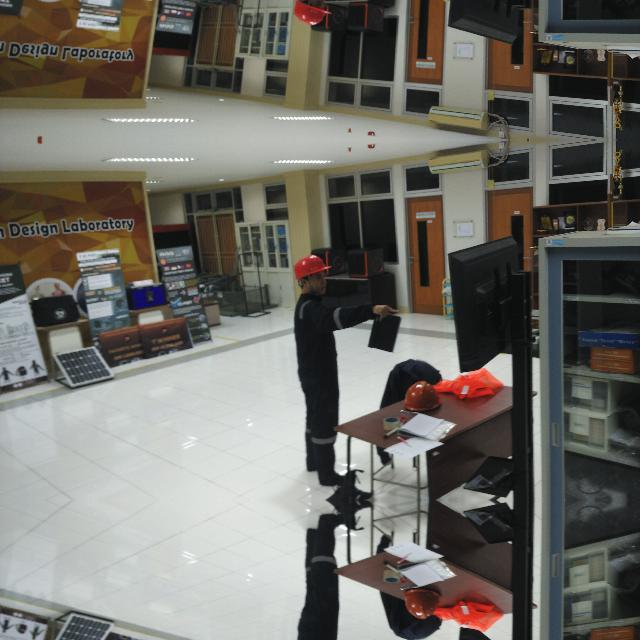
\includegraphics[width=0.3\textwidth]{gambar/sample_erasty/APB-Hat-7-_jpg.rf.4e9ff94579f598546de38a9b5c88a05d.jpg}
    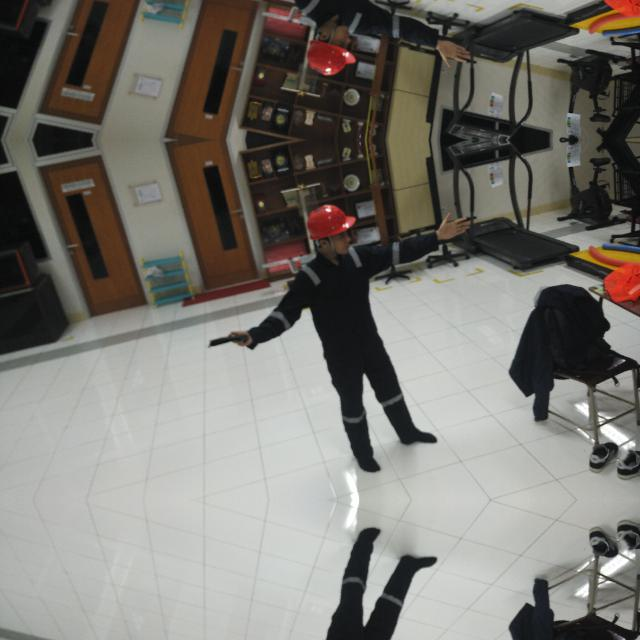
\includegraphics[width=0.3\textwidth]{gambar/sample_erasty/APB-Hat-8-_jpg.rf.804e2e1de8db16912fbbca9d9cfccff3.jpg}
    \caption{Dataset SampleERASTY2020 oleh Muhammad Aditya Wicaksono}
    \label{fig:dataseterastypreview}  
  \end{figure}

\end{enumerate}

\section{Pelabelan Dataset}
\label{sec:pelabelandataset}
Untuk keperluan training dan deteksi, terdapat 2 class :

\begin{enumerate}[nolistsep]
  \item "with\textunderscore helmet" yang meliputi kepala dan helm keselamatan kerja
  \item “no\textunderscore helmet” yang meliputi kepala tanpa helm keselamatan kerja
\end{enumerate}


Pada dataset yang sudah didapatkan sudah memiliki pelabelan atau anotasi nya masing - masing, 
tetapi khusus untuk dataset SampleERASTY2020 terdapat ketidak sesuaian untuk label Hard-hat  
dimana hanya meliputi helm keselamatan kerja tanpa kepala penggunananya. Maka dari itu  dilakukan 
pelabelan ulang untuk dataset SampleERASTY2020 dimana hanya menggunakan file gambar yang masih 
belum hasil augmentasi yang berjumlah 338 gambar. Proses pelabelan gambar dilakukan di platform Roboflow
seperti yang terlihat di Gambar~\ref{fig:gambarbesertalabel}

\begin{figure}[ht]
  \centering
  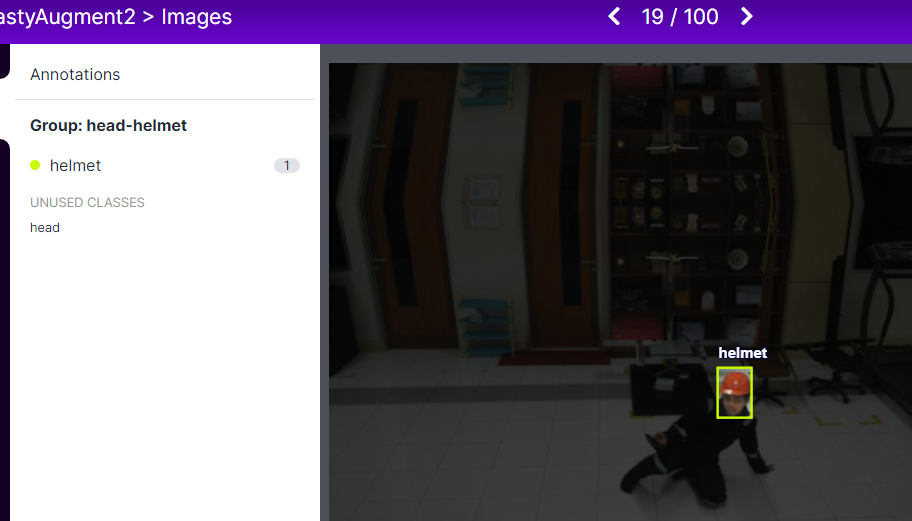
\includegraphics[width=1\textwidth]{gambar/labeldiroboflow.png}
  \caption{Pelabela gambar di Roboflow}
  \label{fig:gambarbesertalabel}  
\end{figure}

\section{Preprocessing Dataset}
\label{sec:preprocessing}
\par Ada beberapa proses yang dilakukan untuk dataset yang sudah dikumpulkan agar bisa digunakan untuk proses
training dengan benar. Proses tersebut meliputi pengaturan ulang ukuran gambar atau \emph{resizing}, penamaan ulang nama kelas, dan augmentasi.
Untuk penelitian ini, proses - proses tersebut dilakukan pada platform Roboflow.


\subsection{Mengatur Ulang Ukuran Gambar}
\par YOLOv5 yang digunakan untuk men-train dataset menerima gambar dalam ukuran 640x640 dengan 
warna RGB sehingga dataset yang ada akan diresize dalam ukuran tersebut. 
Source code YOLOv5 dari repository github sebenarnya sudah menyediakan fitur 
resize sebelum di train tetapi dari penulis melakukan resize menggunakan roboflow. 

\subsection{Membersihkan Dataset}
\par Terdapat beberapa gambar yang tidak diperlukan dari dataset yang didapatkan 
seperti gambar yang hanya memiliki gambar rompi proyek yang dimana tidak digunakan 
untuk keperluan training. Untuk beberapa gambar tersebut akan tidak diikutkan dalam 
export dataset dari roboflow.

\subsection{Penamaan Ulang Nama Kelas Pada Dataset SampleERASTY2020}
\par Penamaan kelas  label yang ada dari dataset yang sudah ada akan disesuaikan untuk 
keperluan penggunaan dan pemahaman yang lebih mudah. Dataset SampleERASTY2020 yang sudah dilabel 
ulang tidak perlu melewati proses ini tetapi untuk dataset Safety Helmet Detection perlu dilakukan 
penamaan ulang dimana untuk class “helmet” menjadi “with\textunderscore helmet” dan “head” 
menjadi “no\textunderscore helmet” seperti yang ditunjukan pada Gambar \ref{fig:prepro_classrename}. 

\begin{figure}[ht]
  \centering
  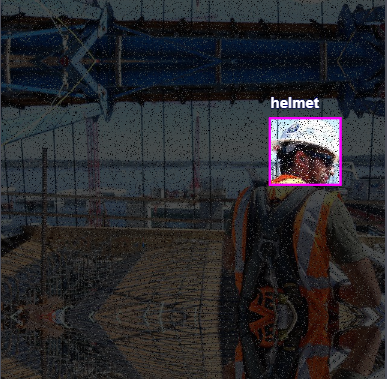
\includegraphics[width=0.4\textwidth]{gambar/reclass_old.png}
  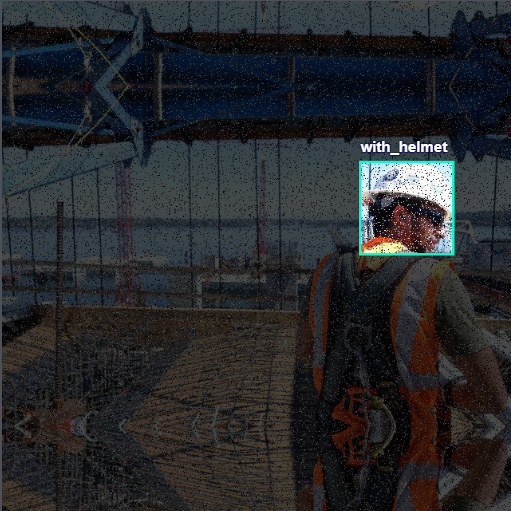
\includegraphics[width=0.4\textwidth]{gambar/reclass_new.png}
  \caption{Nama Kelas Lama dengan Nama Kelas Baru}
  \label{fig:prepro_classrename}  
\end{figure}

\subsection{Augmentasi Gambar}
\par Augmentasi tambahan juga dilakukan pada dataset untuk menambah variasi gambar 
pada dataset dimana untuk bentuk augmentasi yang digunakan yaitu \emph{noise} 
dan \emph{horizontal flip}. Proses augmentasi dilakukan di platform \emph{Roboflow} 
yang juga menyediakan fitur augmentasi. Dataset SampleERASTY2020 yang sudah dilabel 
ulang dan diaugmentasi tambahan lali digabungkan dengan dataset yang sudah 
didapatkan sebelumnya yang berjumlah 5000 gambar. 

\begin{figure}[ht]
  \centering
  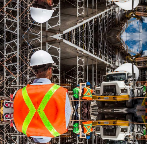
\includegraphics[width=0.4\textwidth]{gambar/aug_flip.png}
  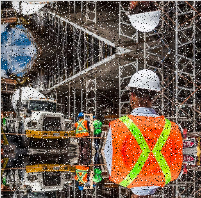
\includegraphics[width=0.4\textwidth]{gambar/aug_noise.png}
  \caption{Augmentasi \emph{Flip} dan \emph{Noise}}
  \label{fig:prepro_augmentasi}  
\end{figure}

% Sebelum di export, dilakukan pembagian rasio file untuk train - test - validation. Pembagian nya yaitu 70\% train (4202) , 20\% test (1.200 gambar), dan 10\% validation (600 gambar). Untuk \emph{training} menggunakan YOLOv5 yang berbasis \emph{PyTorch}, \emph{Roboflow} menyediakan fitur \emph{export} dataset ke format yang ditentukan dimana disini anotasinya disimpan dalam bentuk \emph{.txt} dan diatur lewat file \emph{.yaml}. Lalu khusus untuk dataset SampleERASTY2020 yang sudah dilabel ulang, dilakukan beberapa augmentasi menggunakan roboflow. Augmentasi yang digunakan yaitu flip untuk horizontal dan vertikal diman menghasilkan 600 gambar tambahan. Lalu juga dilakukan augmentasi berupa noise 11\% yang menghasilkan tambahan 300 gambar.

\subsection{Pembagian Dataset}
\par Sebelum digunakan untuk men-\emph{traing} \emph{weight}, dataset yang sebelumnya sudah digabungkan 
perlu ditentukan pembagiannya untuk set \emph{train - test - val}-nya. Pembagian untuk dataset yang 
digunakan untuk training yaitu 70\% train (4202) , 20\% test (1.200 gambar), dan 10\% validation (600 gambar). 
Untuk \emph{training} menggunakan YOLOv5 yang berbasis \emph{PyTorch}, \emph{Roboflow} menyediakan 
fitur \emph{export} dataset ke format yang ditentukan dimana disini anotasinya disimpan dalam bentuk 
\emph{.txt} dan diatur lewat file \emph{.yaml} Pembagian dataset ini dilakukan melalui fitur 
\emph{Generate Dataset Version} pada platform \emph{Roboflow}. Dataset yang didapat dari proses penggabungan dataset
yang disebutkan pada Subbab~\ref{sec:akuisisidataset} dan setelah melalui \emph{pre-processing} selanjutnya akan disebut
sebagai Dataset Helm Keselamatan Kerja untuk mempersingkat.

\begin{longtable}{|c|c|c|}
  \caption{Detail Dataset Deteksi Helm Keselamatan Kerja}
  \label{tb:detailhasilakhirDataset}\\
  \hline
  \rowcolor[HTML]{C0C0C0}
  \textbf{Detail} & \textbf{Keterangan}  \\
  \hline
  Total Gambar & 6.002  \\
  Jumlah \emph{Train Set} & 4.202 \\
  Jumlah \emph{Validation Set} & 1.200\\
  Jumlah \emph{Testing Set} & 600\\ 
  Jumlah label "with\textunderscore helmet" & 19.985 \\
  Jumlah label "no\textunderscore helmet" & 6.601\\
  Resolusi Gambar & 640x640 \\
  \hline
\end{longtable}

\section{Training Dataset}
\label{sec:trainingdataset}

Dataset - dataset yang sudah di pre-process sebelumnya di roboflow dan sudah memiliki anotasi yang susai lalu digunakan untuk training menggunakan YOLOv5. Training ini merupakan proses pelatihan model dengan input gambar - gambar dari dataset yang sudah diberi anotasi dimana gambar dan anotasinya tersebut diolah hingga menghasilkan suatu karakteristik atau pola khusu dari kelas/label yang ditentukan sebelumnya lewat anotasi sehingga selanjutnya dapat digunakan komputer untuk menebak gambar yang nantinya dideteksi. Khusus untuk YOLOv5 yang menggunakan PyTorch sebagai framework machine learningnya, hasil training nya beruba bobot atau weight  akan diexport dalam bentuk .pt (format pytorch). 

\begin{longtable}{|c|c|c|}
  \caption{Konfigurasi Training menggunakan YOLOv5}
  \label{tb:konfigurasitrainingyolov5s}\\
  \hline
  \rowcolor[HTML]{C0C0C0}
  \textbf{Jenis Konfigurasi} & \textbf{Detail}  \\
  \hline
  \emph{batch\textunderscore size} & 16 \\
  \emph{epoch} & 150 \\
  \emph{imgsize} & 640\\
  \emph{data} & /content/yolov5/helmetDetection\textunderscore yolov5\textunderscore 2/data.yaml\\
  \emph{optimizer} & SGD (DEFAULT)\\
  \emph{device} & CUDA\\ 
  \emph{weights} & yolov5n, yolov5s, yolov5m, yolov5l\\ 
  \hline
\end{longtable}


Proses train dilakukan dengan batch size 16 dan 150 epoch dengan optimizer default untuk yolov5 yaitu SGD. Batch\textunderscore size disini menentukan jumlah gambar yang akan digunakan untuk train dalam satu iterasi, ditentukan 16 dengan pertimbangan limitasi hardware yang digunakan untuk proses training ini. Proses training dilakukan di Colab Pro dimana dengan limitasi GPU Ram yang diberikan, digunakan hingga mendekati 12 GB. Untuk image size sendiri algoritma yang sudah disediakan oleh YOLOv5 hanya menyiadakan resolusi 1:1 dimana dengan mengeset parameter imgsize 640 berarti ukuran untuk \emph{(height)} dan \emph{(width)} menjadi 640x640.

Proses training untuk judul ini tidak dilakukan dengan hardware komputer lokal melainkan memanfaatkan Google Colab Pro dimana proses trainingnya dijalankan secara cloud. 
Dataset yang sudah dikumpulkan sebelumnya didownload ke storage vm Colab Pro langsung dari Roboflow.  Dengan limitasi penggunaan storage, ram, dan GPU ram serta runtime yang diberikan google colab, dilakukan penyimpanan checkpoint untuk tiap epoch training di drive pribadi penulis. Hal dilakukan untuk kemungkinan jika sekiranya di tengah proses training session VM Colab Pro nya ter -terminate dengan sendirinya. 


\section{Perancangan Sistem Deteksi Helm Keselamatan Kerja}
\label{sec:perancangansistem}

\begin{figure}[ht]
  \centering
  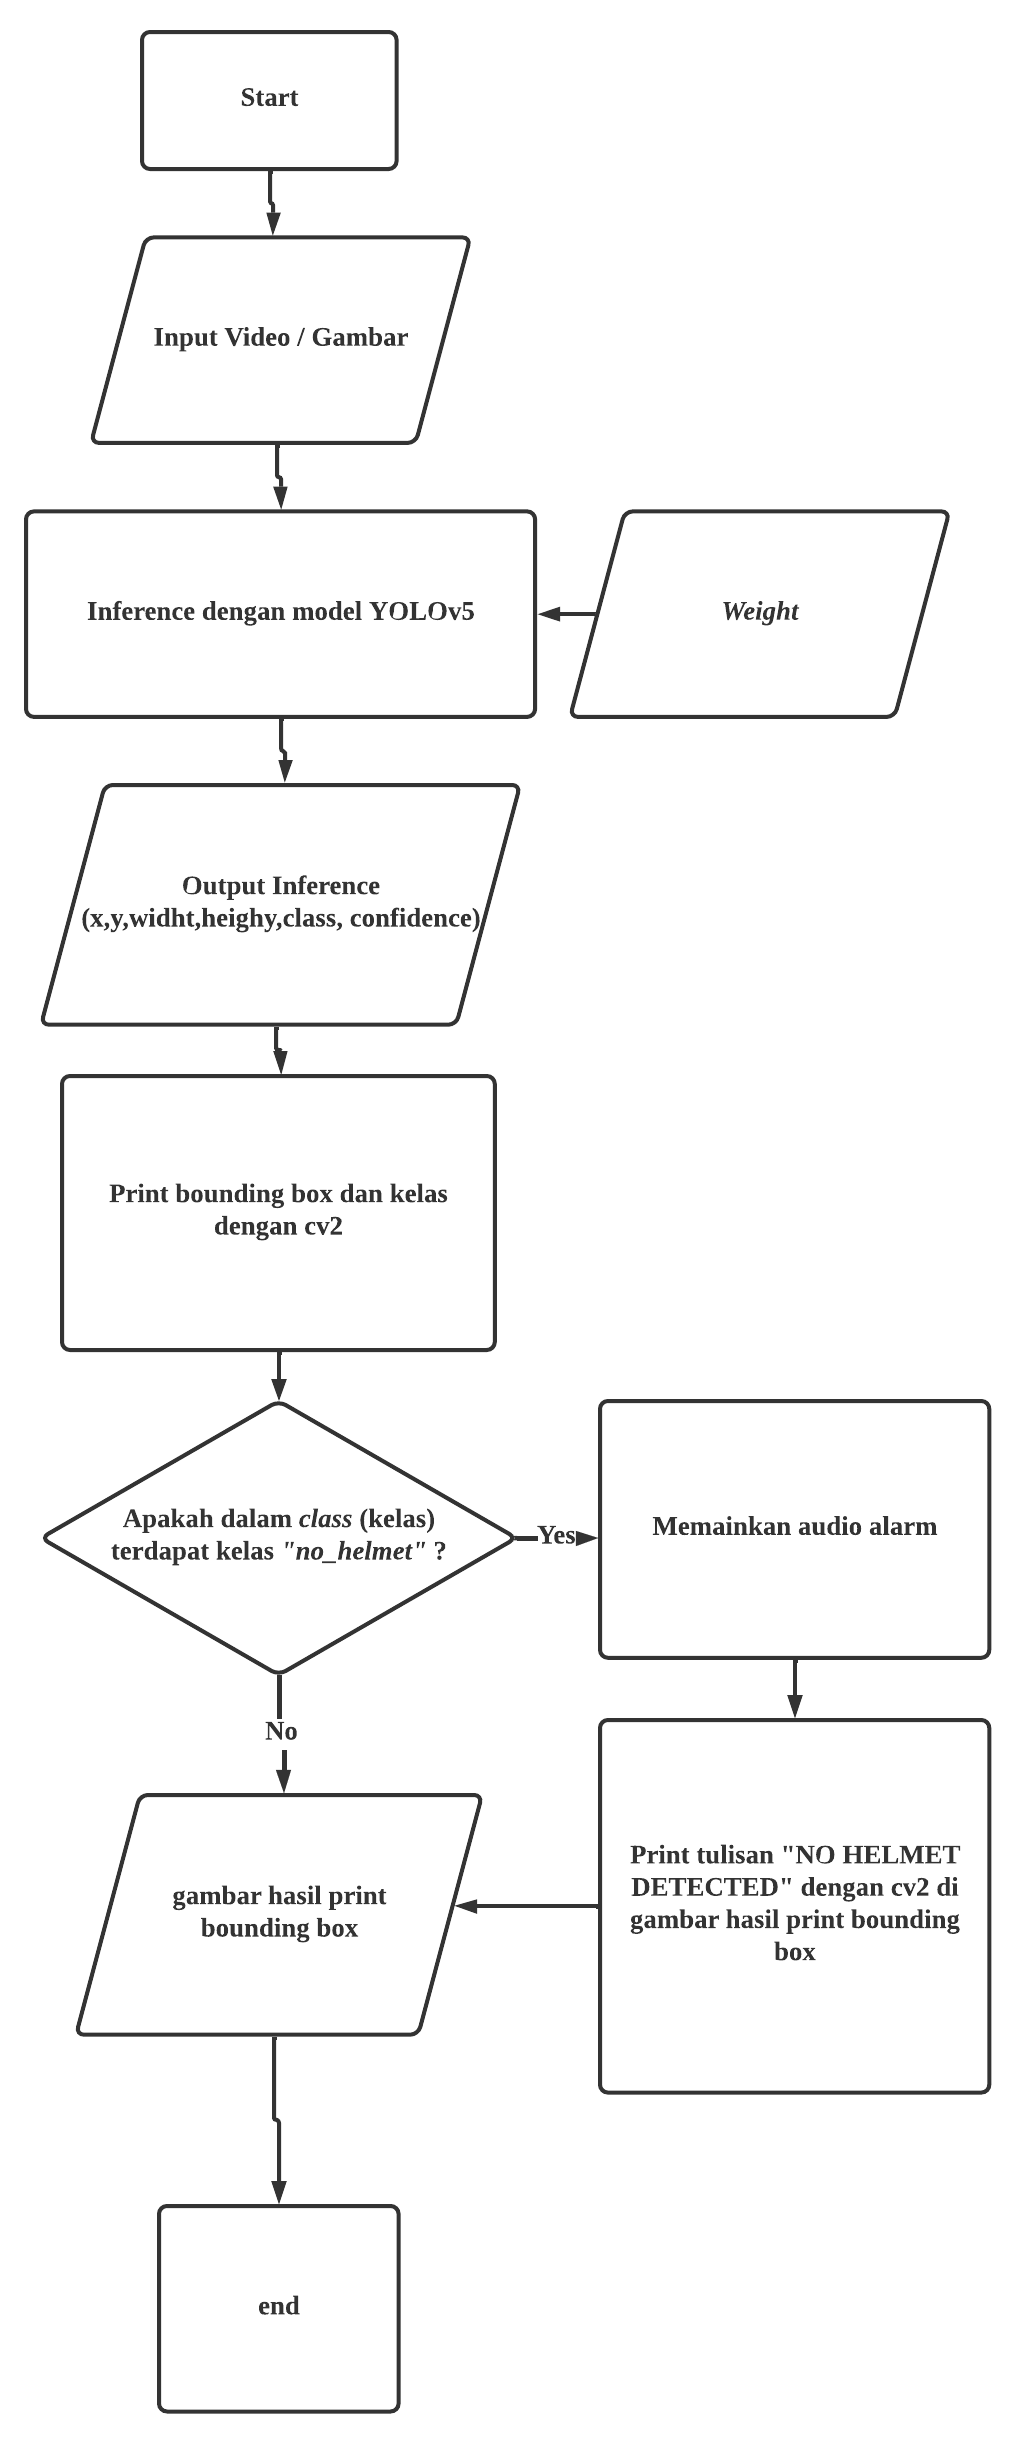
\includegraphics[scale=0.55]{gambar/flowchart_sistemhedec.png}
  \caption{Flowchart Sistem Deteksi Helm Keselamatan Kerja}
  \label{fig:flchartdeteksi}  
\end{figure}

Sistem deteksi yang dibuat untuk Deteksi Helm Keselamatan kerja sendiri dikembangkan dari sistem deteksi yang sudah ada dari YOLOv5 dengan beberapa perubahan yang disesuaikan khusus untuk judul ini. Flowchart untuk sistem Deteksi Helm Keselamatan Kerja dapat dilihat pada Gambar~\ref{fig:flchartdeteksi} .

% Sistem yang dibuat direncanakan akan dijalankan di komputer yang sudah terinstall Python dan framework PyTorch atau ONNX dimana merupakan format yang dihasilkan dari training sebelumnya.

Sistem nya akan dibuat sebagai file script python yang dapat di run dan dapat menerima beberapa parameter : ukuran gambar, sumber input, dan bobot atau weight yang akan digunakan. 
Input yang dapat digunakan dengan script yang dibuat dapat dilakukan dalam bentuk gambar, file video, link youtube, link stream, dan feed camera dengan basis dari script detect.py dari YOLOv5. Tetapi, yang akan digunakan sebagai default nanti adalah feed dari kamera atau webcam yang tersedia di hardware yang digunakan untuk menjalankan inference. Ukuran atau resolusi gambar yang diterima sebagai ukuran default yaitu 640x640. 

% Untuk kasus jika input berupa gambar tunggal, gambar tersebut akan digunakan untuk inference melalu model yolov5 dengan bobot yang sudah dibuat sebelumnya lalu hasil inference yolov5 akan menghasilkan beberapa output. Tetapi untuk sistem yang akan dijalankan akan memanfaatkan feed dari camera atau webcam secara realtime sehingga akan dilakukan inference untuk tiap frame yang masuk dari input webcam.

\par Tiap frame yang masuk dari input \emph{webcam} akan digunakan untuk proses \emph{inference} melalui 
model \emph{yolov5} dengan \emph{weight} yang sudah dibuat sebelumnya melalui proses training. 
Hasil dari \emph{inference} menggunakanm \emph{YOLOv5} akan menghasilkan input berupa posisi untuk 
objek yang dideteksi yaitu \emph{xcenter, ycenter} serta dimensi dari objeknya yaitu \emph{widht} 
dan \emph{height} serta informasi nama \emph{class} dan \emph{confidence\textunderscore score} untuk 
tiap objek yang dideteksi. Hasil \emph{output inference} yang didapat lalu digunakan untuk menggambar 
\emph{bounding box} pada \emph{frame} gambar yang sedang di\emph{inference} 
seperti pada Gambar~\ref{fig:outputboundingbox}.

\begin{figure}[ht]
  \centering
  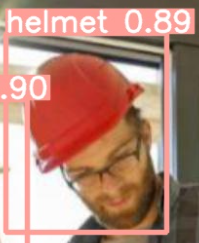
\includegraphics[scale=1]{gambar/bounding_box.png}
  \caption{Output Bounding Box}
  \label{fig:outputboundingbox}
\end{figure}

% Output yang dikeluarkan dari hasil inferensi menggunakan yolov5 yaitu xcenter, ycenter, width , height, confidence, dan class. Untuk keperluan menampilkan bounding box akan menggunakan xcenter, ycenter, width, dan height yang didapatkan dari output inference yang lalu dilengkapi dengan menampilkan nama class dan confidence score dari inferencenya. 

% Untuk fungsi trigger alarm jika terdeteksi adanya orang yang tidak menggunakan helm, untuk hasil output yang dihasilkan dari inference satu frame akan dicheck sekiranya mengandung class “no\textunderscore helmet” yang jika terpenuhi akan  menjalankan perintah untuk mengeprint “NO HELMET DETECTED” pada display dan menjalankan audio alarm. 

\par Fungsi alarm akan dijalankan ketika dalam frame yang sedang di-\emph{inference} terdeteks objek 
dengan \emph{class} bernama \emph{“no\textunderscore helmet”}. Fungsi alarm ini berisi perintah untuk 
memainkan audio alarm untuk mensimulasikan sirine alarm. Selain menjalankan fungsi alarm, akan juga 
dijalanan perintah untuk mendisplay text \emph{“NO HELMET DETECTED”} pada frame yang sedang 
di-\emph{inference} seperti yang ditunjukan pada Gambar~\ref{fig:deteksinohelm}.

\begin{figure}[ht]
  \centering
  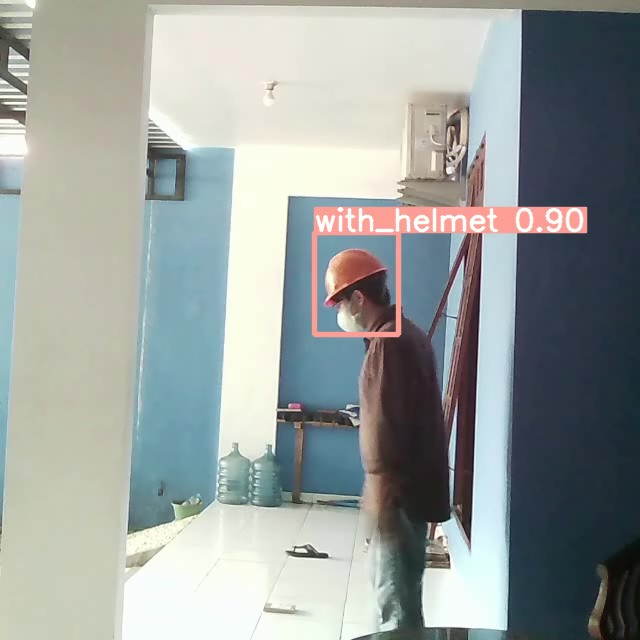
\includegraphics[scale=0.3]{gambar/video2_Moment.jpg}
  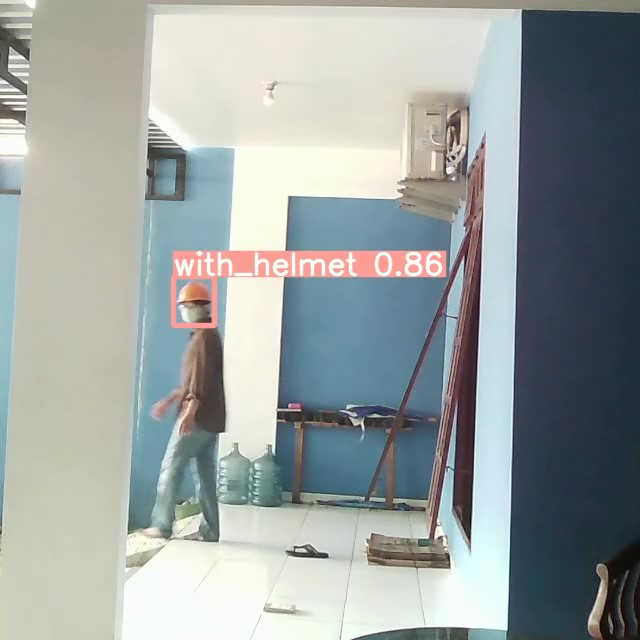
\includegraphics[scale=0.3]{gambar/video2_Moment2.jpg}
  \caption{Proses Deteksi Menggunakan Helm Keselamatan Kerja}
  \label{fig:deteksiwthhelm} 
\end{figure}

\begin{figure}[ht]
  \centering
  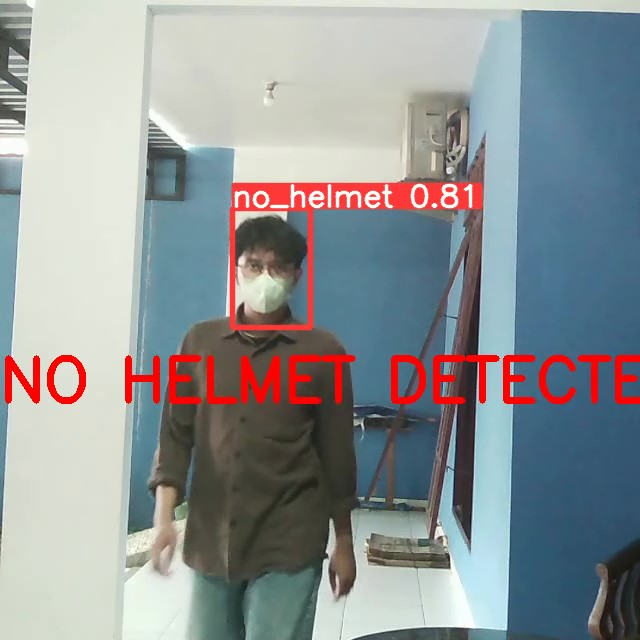
\includegraphics[scale=0.3]{gambar/video1_Moment.jpg}
  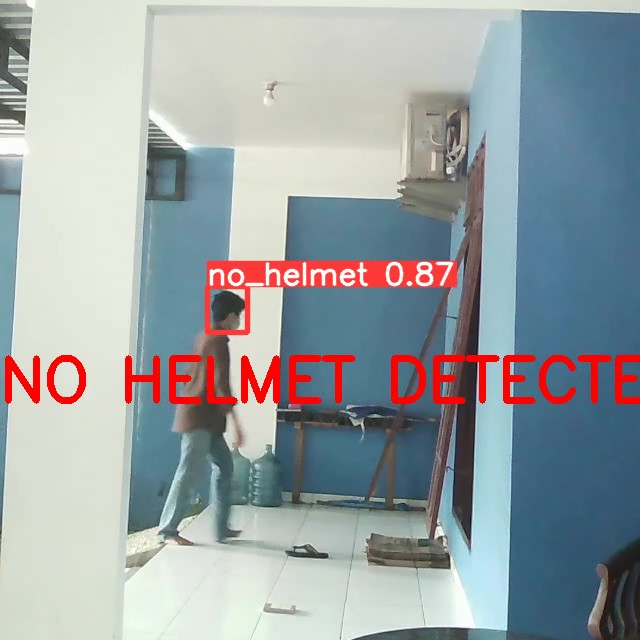
\includegraphics[scale=0.3]{gambar/video1_Moment2.jpg}
  \caption{Proses Deteksi Tidak Mengenakan Helm Keselamatan Kerja}
  \label{fig:deteksinohelm}  
\end{figure}

% Per blok diagram dijelaskan dan dibuatkan section masing-masing

% \section{Blok Diagram}
% \label{sec:blokdiagram}

% Contoh pembuatan potongan kode
% \begin{lstlisting}[
%   language=C++,
%   caption={Program halo dunia.},
%   label={lst:halodunia}
% ]
% #include <iostream>

% int main() {
%     std::cout << "Halo Dunia!";
%     return 0;
% }
% \end{lstlisting}

% \lipsum[2-3]

% % Contoh input potongan kode dari file
% \lstinputlisting[
%   language=Python,
%   caption={Program perhitungan bilangan prima.},
%   label={lst:bilanganprima}
% ]{program/bilangan-prima.py}

% \lipsum[4]
